\section{Users Tab}
\subsubsection{Overview}
The \textbf{Users tab} allows the user to view and edit existing user's information and allocate them to particular campuses. 

\begin{figure}[H]
    \centering
    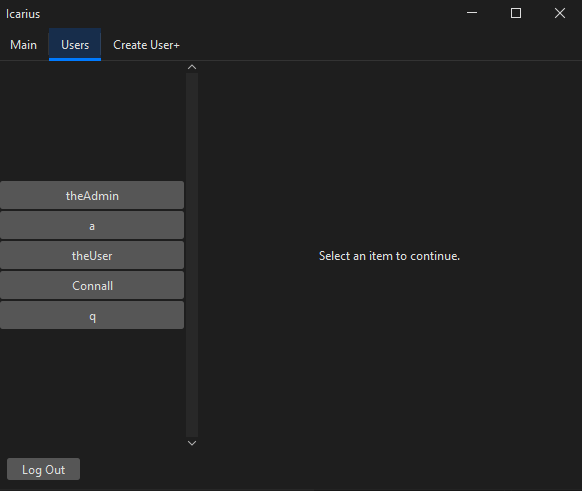
\includegraphics[width=0.6\textwidth]{UsersTab/usersTabOverview.PNG}
\end{figure}

\subsubsection{Viewing an existing user}
In order to view an existing user, the user must:
\begin{enumerate}
    \item Click on a user located in the left panel of the tab. \textit{This will reveal the attributes of that user on the right}
    \begin{figure}[H]
        \centering
        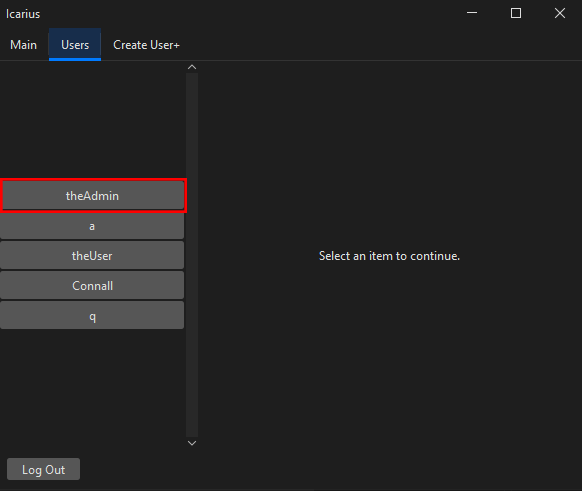
\includegraphics[width=0.6\textwidth]{UsersTab/viewUser/viewUser.png}
        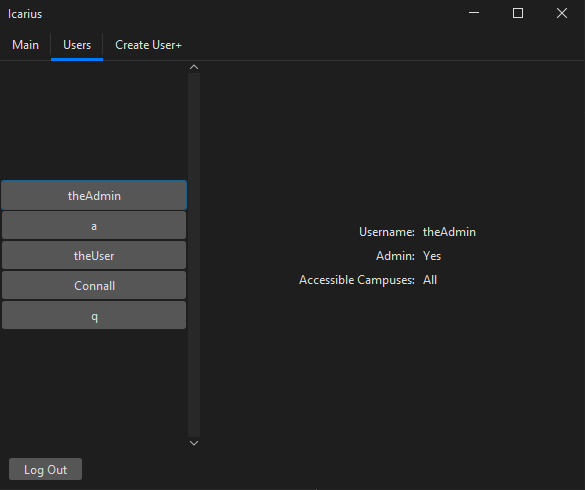
\includegraphics[width=0.6\textwidth]{UsersTab/viewUser/viewUserSelected.png}
    \end{figure}
    The attributes of a user are as follows:
    \begin{itemize}
        \item \textbf{Username:} The selected users username
        \item \textbf{Admin:} Displays whether the user is an admin or not
        \item \textbf{Accessible Campuses:} A list of all of the campuses the user is able to make edits to within the main tab. If the selected user is an admin this will just say \textbf{All}
    \end{itemize}
\end{enumerate}

\subsubsection{Editing an existing user}
Admin users cannot have their attributes be changed.

In order to edit an existing user, the user must:
\begin{enumerate}
    \item Click on a user located in the left panel of the tab.  \textit{This will reveal the attributes of that user on the right}
    \begin{figure}[H]
        \centering
        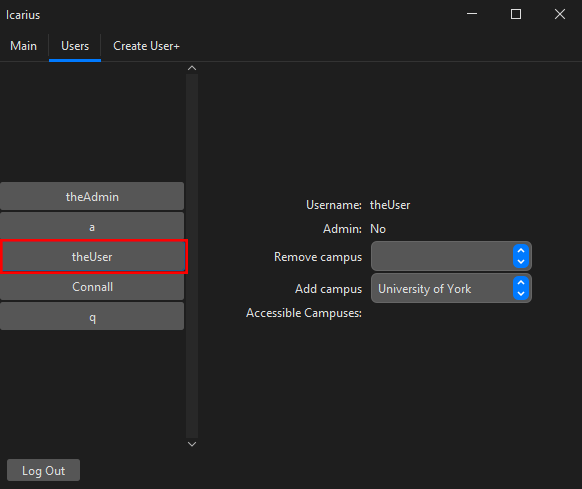
\includegraphics[width=0.6\textwidth]{UsersTab/editUser/editUser.png}
    \end{figure}

    \item A campus can be added to the user by clicking on the \textbf{Add Campus} drop-down list. \textit{This will reveal each campus in the database}
    \begin{figure}[H]
        \centering
        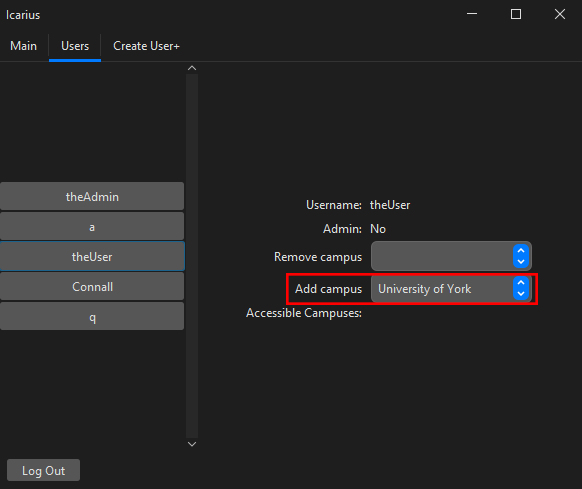
\includegraphics[width=0.6\textwidth]{UsersTab/editUser/editUserAdd.png}
        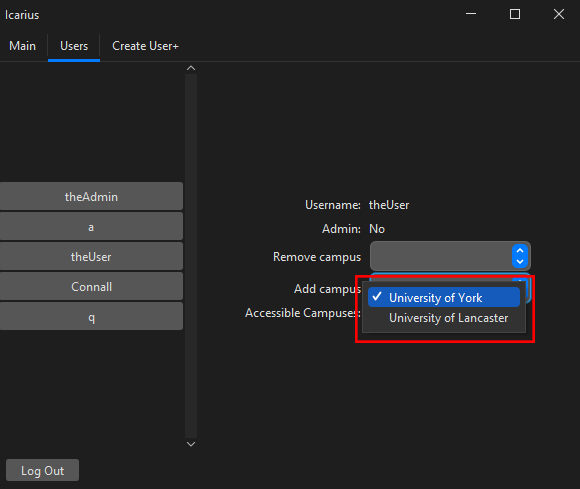
\includegraphics[width=0.6\textwidth]{UsersTab/editUser/editUserAddView.png}
    \end{figure}
    
    Similarly, a campus can be removed from the user by clicking on the \textbf{Remove Campus} drop-down list.
    \begin{figure}[H]
        \centering
        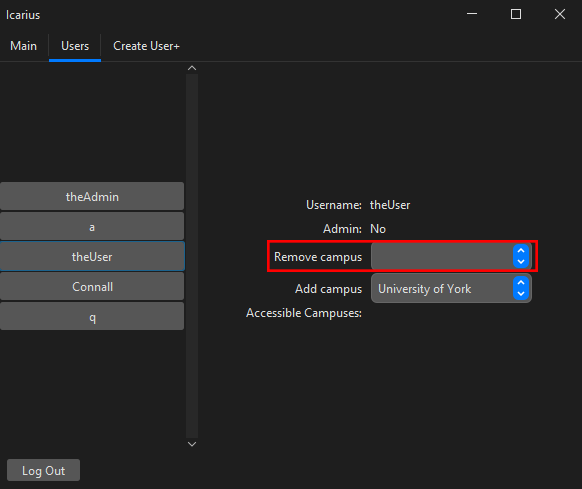
\includegraphics[width=0.6\textwidth]{UsersTab/editUser/editUserRemove.png}
        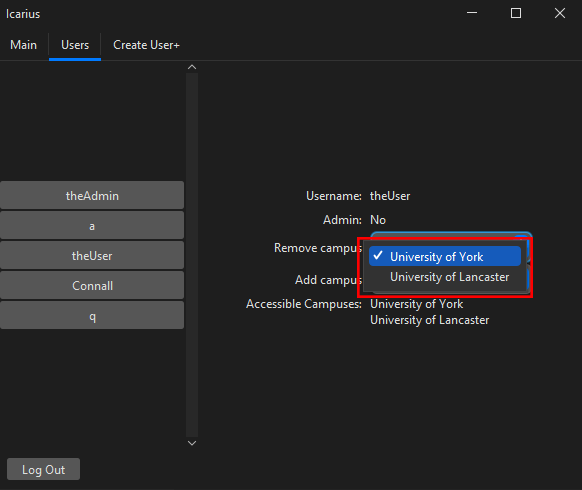
\includegraphics[width=0.6\textwidth]{UsersTab/editUser/editUserRemoveView.png}
    \end{figure}
\end{enumerate}